\documentclass[11pt,letterpaper,boxed]{../hmcpsetrhino}
\usepackage[margin=1in]{geometry}
\usepackage{graphicx}
\usepackage{enumerate}
\usepackage{amsthm}
\usepackage{amsmath}

\newcommand{\ds}{\displaystyle}
\newcommand{\half}{\frac{1}{2}}
\newcommand*\Eval[3]{\left.#1\right\rvert_{#2}^{#3}}
\newcommand{\eval}{\biggr\rvert}
\newcommand\Partial[2]{\frac{\partial #1}{\partial #2}}
\let\oldvec\vec
\renewcommand{\vec}[1]{\oldvec{\mathbf{#1}}}
\def\EE{{\cal E}}
\def\Lagr{\mathcal{L}}
\def\Ham{\mathcal{H}}

\name{}
\class{Physics 111 Section 1}
\assignment{Problem Set 09}
\duedate{October 10, 2016}

\begin{document}

\problemlist{Noninertial Frames (Reading: Chapter 9.1 - 9.5)}
\textbf{Help:} 

\begin{problem}[i]
Follow Taylor's presentations in section 9.4 and re-derive equation 9.30. As usual, my intent here is not to have you blindly follow Taylor's presentation but to really understand and internalize the derivation that leads us to 9.30.
\end{problem}
\begin{solution}


\vfill
\end{solution}

\newpage 

\begin{problem}[9.6]
Let $h(\theta)$ denote the height of the ocean at any point $T$ on the surface, where $h(\theta)$ is measured up from the from the level at the point $Q$ of Figure 9.5 and $\theta$ is the polar angle $TOR$ of $T$. Given that the surface of the ocean is an equipotential, show that $h(\theta) = h_0 \cos^2\theta$, where $h_0 = 3 M_m {R_e}^4 / (2M_e {d_0}^3)$. Sketch and describe the shape of the ocean's surface, bearing in mind that $h_0 \ll R_e$. [\textit{Hint}: You will need to evaluate $U_{tid}(T)$ as given by 9.13, with $d$ equal to the distance $MT$. To do this you need to find $d$ by the law of cosines and then approximate $d^{-1}$ using the binomial approximation, being very careful to keep \textit{all} terms through order $(R_e/d_0)^2$. Neglect any effects of the sun.]
\[	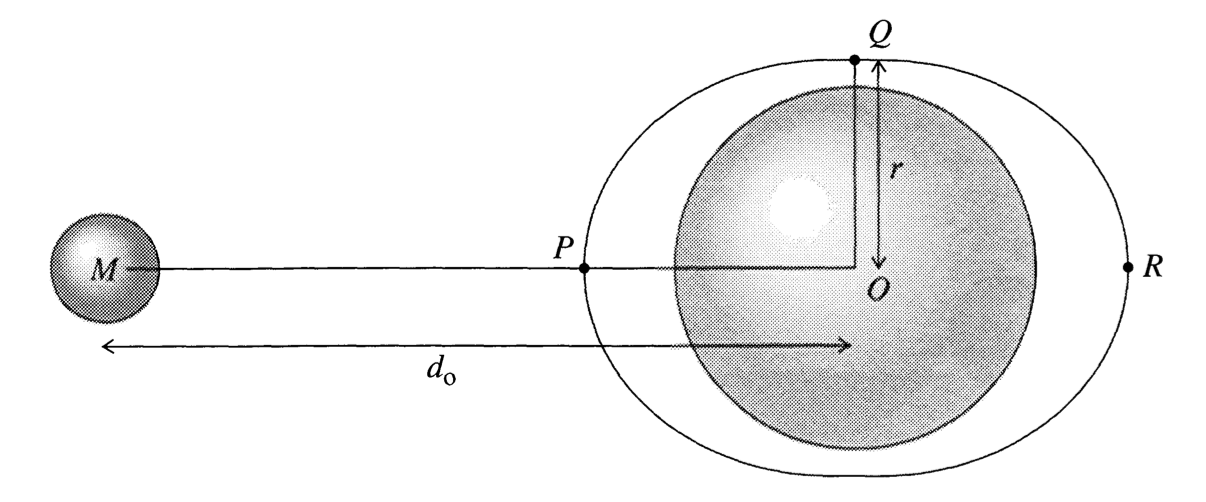
\includegraphics[width=\textwidth]{fig1}\]
\end{problem}
\begin{solution}


\vfill
\end{solution}


\newpage

\begin{problem}[9.11]
In this problem you will prove the equation of motion (9.34) for a rotating frame using the Lagrangian approach. As usual, the Lagrangian method is in many ways easier than the Newtonian (except that it calls for some slightly tricky vector gymnastics), but is perhaps less insightful. let $\mathcal{S}$ be a non inertial frame rotating with constant angular velocity $\vec \Omega$ relative to the inertial frame $\mathcal{S}_0$. Let both frames have the same origin, $O = O'$.
\begin{enumerate}[(a)]
\item Find the Lagrangian $\mathcal{L} = T-U$ in terms of the coordinates $\vec r$ and $\dot {\vec r}$ of $\mathcal{S}$. [Remember that you must first evaluate $T$ in the inertial frame. In this connection, recall that $\vec v_0 = \vec v + \vec \Omega \times \vec r$.] 
\item Show that the three Lagrangian equations reproduce 9.34 precisely.
\end{enumerate}
\vspace{0.2cm}
\hspace{1.5cm}\hfill $m\ddot {\vec r} = \vec F + 2 m \dot{\vec r} \times \vec \Omega + m(\vec \Omega \times \vec r) \times \vec \Omega$\hfill (9.34)
\end{problem}
\begin{solution}


\vfill
\end{solution}

\end{document}
